\section{Theory}
	
	%order:
	%reservoir condition - fading memory etc.



	\subsection{Stuart-Landau-Oscillator}
	The Stuart-Landau oscillator is a dynamical system often used to model basic class 1 lasers. It can be written either as a single complex differential equation (\ref{eq:stuartlandauequation}) or a set of two equations written in polar coordinates (\ref{eq:stuartlandauequation_polar}). From the equation in polar coordinates easy to see that the equation has rotational symmetry as the radial differential equation does not change with the dynamical variable $\phi$.
	
	\begin{equation}	
		\dot{z} = (\lambda +  i \omega + \gamma |z|^2 ) \; z
		\label{eq:stuartlandauequation}		
	\end{equation}
	
	\begin{equation}
		\begin{split}
		\dot{r} & = \lambda r + \operatorname{Re} (\gamma) \; r^{3} \\
		\dot{\phi} &= i \omega + \operatorname{Im}(\gamma) \; r^{2} 
		\end{split}
		\label{eq:stuartlandauequation_polar}
	\end{equation}

	For the radial dynamical variable the Stuart-Landau oscillator has two fixed points where the derivative $\dot{r}$ vanishes $r = 0$ and $r = \sqrt{-\lambda /\operatorname{Re}(\gamma)}$ whose stability depends on $\lambda$ and $\operatorname{Re}(\gamma)$. For $\operatorname{Re}(\gamma) < 0 $ (supercritical case).
	

	\begin{figure}
		\centering
		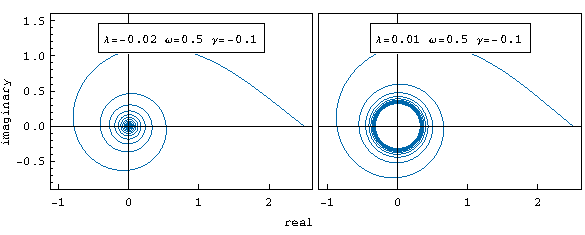
\includegraphics[width=0.99\linewidth]{pics/stuart_landau_complex_Focus_LC}
		\caption{$2$ very basic scenarios of the Stuart-Landau oscillator: Decay towards a single fixed point (left) or towards a limit cycle (right).}
		\label{fig:stuart_spiral}
		%nicht mehr
		%stuart_landau_basic.nb
	\end{figure}



The limit cycle (LC) which is shown in fig \ref{fig:stuart_spiral} is depending on the ratio or $\lambda$ and $Re \left[\gamma \right]$.





As can be seen in (eq. \ref{eq:stuartlandauequation}), the equation has a linear and a nonlinear term regarding the absolute value of $z$.

\subsection{Networks}

Vertices blabla \
Edges blabla. \

	\subsubsection{circulant Matrix}
    A circulant matrix has the same entries its row vectors, but with its entries rotated one element to the right relative to the previous row.
    
\subsection{virtual Nodes and multiplexing}
	here: papers for explanation! 
	\cite{KUR18}
	
	\cite{STE20} // off-resonance = better! --> reason for choosing 17 * 12.
	
	By multiplexing the input signal one can create virtual nodes in a network. The analogy to a real network can be best understood if the input signal is masked with a binary mask containing only values of either $0$ or $1$. 
	
	Different Mask types: discrete values with constant interpolation: binary, uniform - easy to implement)
	continuous: any function or repeating noise-patterns. (more difficult, but )
	
	
	here add dependency of total linear memory on number of nodes and virtal nodes.
	
	
	\begin{figure}
		\centering
		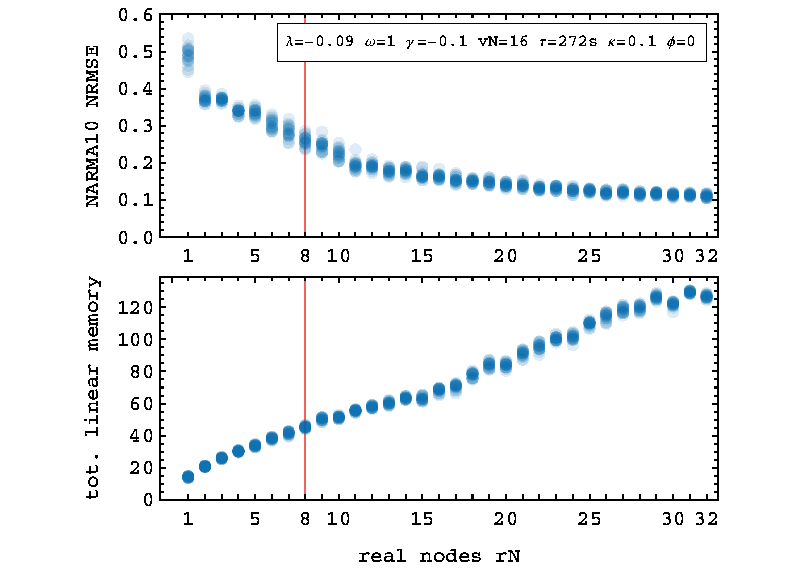
\includegraphics[width=0.9\linewidth]{pics/rNplot}
		\caption{changing rc performance for increasing number or real nodes $rN$ in unidirectianally coupled ring networks. (see some plot).}
		\label{fig:rN_1-32}
	\end{figure}

	\begin{figure}
	\centering
	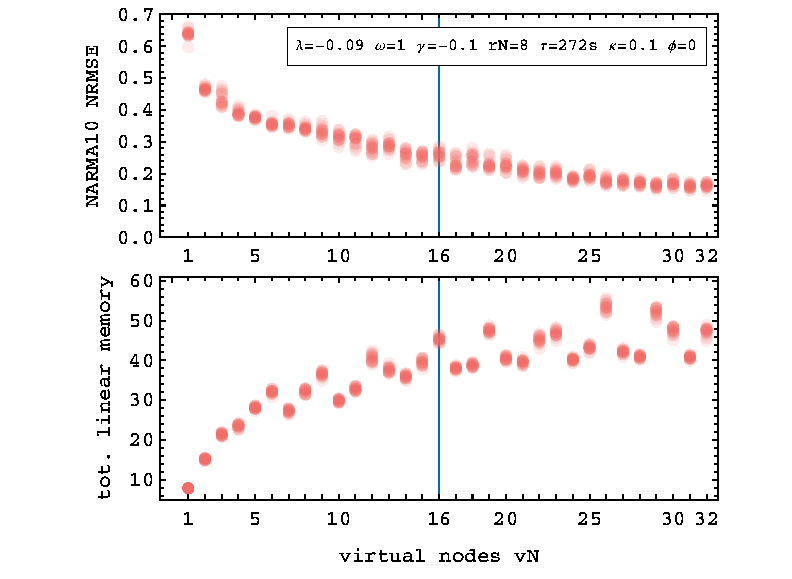
\includegraphics[width=15cm]{pics/vNplot}
	\caption{changing rc performance for increasing number or virtual nodes $rN$ in unidirectionally coupled ring networks. (see some plot).}
		\label{fig:vN_1-32}
	\end{figure}


\begin{figure}
	\centering
	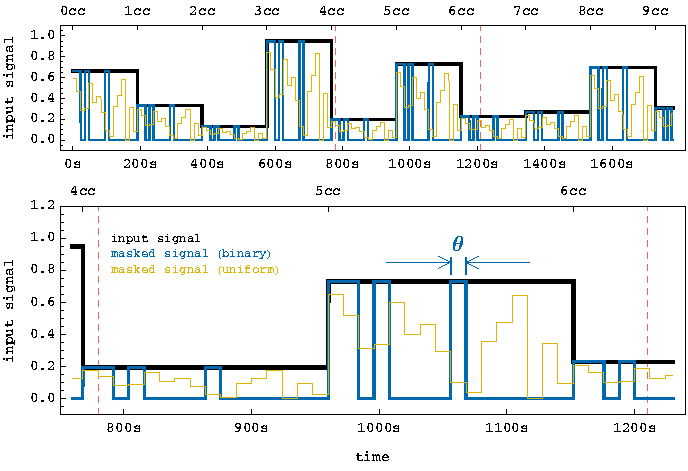
\includegraphics[width=15cm]{pics/signal_mask_vis}
	\caption{A timeseries (black) with constant interpolation ("sample \& hold") between samples and the corresponding masked signal (blue). The mask length is counted in clockcycles (cc) and the time per virtual node is counted in $\theta$. Here $\theta = 12s$ and $1cc = 16 \theta = 272s $}
	\label{fig:signal_mask_vis}
	%feedInVis_stuartlandau.nb
\end{figure}

	

\subsection{Dynamics of rings of stuart landau oscillators}
	pony-states (von André)
	
\subsection{Reservoir computing}
	
	\subsubsection{Measuring computation performance}
	We can measure how well a dynamical system perform computations by testing it in a variety of benchmarks. Dynamical systems are continuously evolving in time, thus reservoir computation mostly is mostly tested on timeseries data. There exist also approaches of using RC on datasets that do not involve datasets without a temporal dimension e.g. image classification of single images \cite{}
	
	
	
	
\subsection{Reservoir computing tasks}
	The reservoir computing performance of a given reservoir can be quantified by testing its predictions for certain tasks. In machine learning the task is usually to predict a certain value or set of values from an input set of inputs. Ideally the prediction can then be compared to the base truth and the difference between prediction and base truth is used to quantify the error. The closer the prediction is to the ground truth, the better the system 
	performs a given task. It is important to note that usually these predictions always aren't singular, but give a vector of probabilities. A neural network used for image classification will output a vector with probabilities e.g. it is quantifying the "dog-ness", the "tree-ness" or the "car-ness" of an input image. The actual decision is made by choosing the entry with the highest probability. 
	For predictions based on timeseries data the same applies. They are represented by continuous values that the system puts out.  
	

	

\subsubsection{Linear Memory Recall}
	The simplest task a reservoir can perform is to repeat the the information that was fed into it at a certain point in time.  


	\begin{figure}
	\centering
	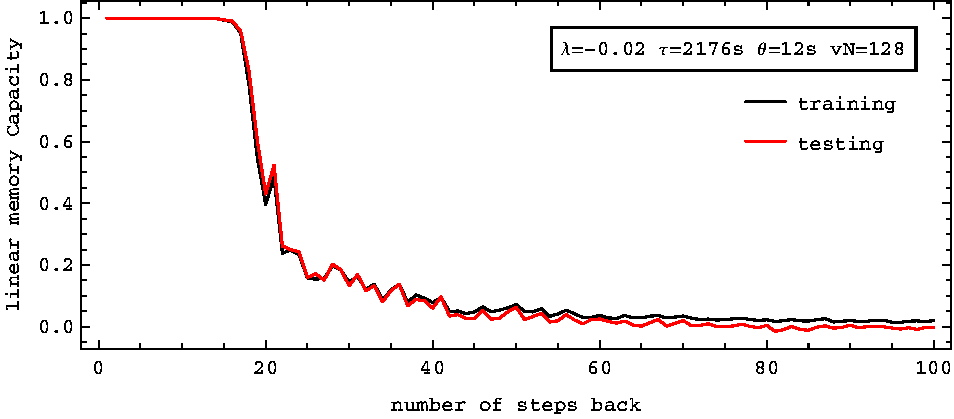
\includegraphics[width=0.99\linewidth]{pics/linearMemoryCurveN1}
	\caption{The linear memory capacities for differently many steps into the past. The system is able to perfectly reproduce inputs up until $12$ steps into the past. $N=1, vN=128, \lambda=-0.02, \omega=1, \gamma=-0.1, \theta=12, \tau=2176$. }
	\label{fig:linearMemoryRecallCurveN1}
	\end{figure}


\subsubsection{NARMA10 NRMSE}

	

% different stuart landau scenarios - hopf bifurcation